%%%%%%%%%%%%%%%%%%%%%%%%%%%%%%%%%
% ammana.es | Manual de cliente %
%                               %
%  Made with ❤️  by NoLegalTech  %
%%%%%%%%%%%%%%%%%%%%%%%%%%%%%%%%%

\documentclass[12pt, spanish]{article}

\usepackage{geometry}
\geometry{a4paper}

\usepackage{graphicx}
\graphicspath{{img/}}

\usepackage{adjustbox}

\usepackage{float}
\usepackage{wrapfig}

\usepackage[spanish]{babel}
\selectlanguage{spanish}

\usepackage[utf8]{inputenc}

\usepackage{enumitem}

\linespread{1.2}

\setlength{\parindent}{2em}
\setlength{\parskip}{1em}

\usepackage{concmath}
\usepackage[T1]{fontenc}

\usepackage{fancyhdr}

\fancyhf{}
\fancyhead[L]{
\includegraphics[height=5.0mm]{logo}}

\usepackage{hyperref}
\hypersetup{
    colorlinks=true,
    linkcolor=[rgb]{0.25,0.55,0.79},
    filecolor=magenta,
    urlcolor=[rgb]{0.25,0.55,0.79},
}

\newlist{steps}{enumerate}{1}
\setlist[steps]{label={\arabic*)}}

\setlength{\headheight}{7.50mm}
\pagestyle{fancy}

%----------------------------------------------------------------------------------------

\begin{document}

%----------------------------------------------------------------------------------------

    \begin{titlepage}
        \newcommand { \HRule } { \rule {\linewidth} {0.5mm} }
        \center
        \textsc {\LARGE ammana.es} \\ [1.5cm]
        \HRule \\ [0.4cm]
        { \huge \bfseries Manual del administrador } \\ [0.4cm]
        \HRule \\ [1.5cm]
        { \large \today } \\ [3cm]
        \vfill
    \end{titlepage}

%----------------------------------------------------------------------------------------

    \tableofcontents

    \newpage

%----------------------------------------------------------------------------------------

    \section{Introducción}

        Este manual pretende servir de guía al administrador de \textbf{ammana.es} para 
    realizar sus funciones, así como comprender las funciones de los clientes y poder, en
    su caso, darles el soporte adecuado.

        El manual está separado en 2 grandes secciones. La primera de ellas cubre las funciones
    específicas del administrador, y la segunda las que el resto de usuarios (clientes) pueden
    realizar.

        Completamos ahora esta introducción con información básica sobre las urls y cuentas de
    usuario de \textbf{ammana.es}.

%----------------------------------------------------------------------------------------

    \subsection{URLs}

        ammana está publicado en \url{ammana.es}

        También existen las siguientes {\em landing pages}:
        \begin{itemize}
            \item \url{protocololaboral.com}
            \item \url{protocololaboral.es}
        \end{itemize}

%------------------------------------------------

    \subsection{Cuentas de usuario}

        Cada cliente tiene una única cuenta de usuario y podrá acceder a la página usando
    sus credenciales (email + contraseña).

        Los clientes se pueden (y deben) registrar ellos mismos (ver \hyperref[sec:registro]{Registro}).
    
        Existe además la cuenta de administrador, que es única (no se pueden registrar
    más cuentas de administración). Como administrador, accederás al panel de administración
    usando el mismo proceso de \hyperref[sec:login]{Identificación} que los clientes, pero con
    tus credenciales de administrador.

%----------------------------------------------------------------------------------------

    \section{Funciones del administrador}

            \textbf{ammana.es} funciona de forma prácticamente autónoma y los clientes pueden
        comprar y descargar protocolos sin intervención del administrador. La única
        excepción es cuando algún cliente paga por transferencia bancaria, en cuyo
        caso el pago debe ser marcado como cobrado de forma manual para que el cliente
        pueda descargarse el protocolo.

            Por otro lado, el panel de administración de \textbf{ammana.es}, junto con los de
        \textbf{Paypal} y \textbf{Quaderno}, dan acceso al administrador a la lista de clientes,
        facturas, pedidos, etc para su consulta, bien por curiosidad bien para ofrecer soporte
        a un cliente..

        Es decir, las funciones del administrador son 2:

        \begin{steps}
            \item Marcar como cobrados los pedidos que han sido pagados por transferencia
            \item Acceder a la información de clientes y facturas
        \end{steps}

%----------------------------------------------------------------------------------------

    \section{Funciones del cliente}

            Los clientes de \textbf{ammana.es} pueden registrarse, comprar protocolos y 
        descargarlos sin intervención del administrador.

            Además de descargar protocolos, pueden ver instrucciones de los mismos y descargar
        modelos de ``recibí'', ver sus facturas o modificar su perfil.

        Es decir, las funciones del cliente son:

        \begin{steps}
            \item Gestionar su cuenta (registro, identificación, datos de perfil, ...)
            \item Acceder a la información de clientes y facturas
        \end{steps}

%----------------------------------------------------------------------------------------

    \subsection{Gestión de cuenta}

%----------------------------------------------------------------------------------------

    \subsubsection{Registrarse}

    \label{sec:registro}

    \begin{steps}

        \item Clic en ``Registrarse'' en el menú superior:

            \medskip
            \begin{minipage}[t]{\linewidth}
            \raggedright
            \adjustbox{valign=t}{%
                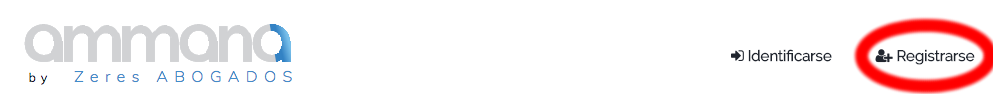
\includegraphics[width=1\linewidth]{register/1.png}
            }
        \end{minipage}

        \item Introducir email y contraseña en el formulario de registro:

            \medskip
            \begin{minipage}[t]{\linewidth}
            \raggedright
            \adjustbox{valign=t}{%
                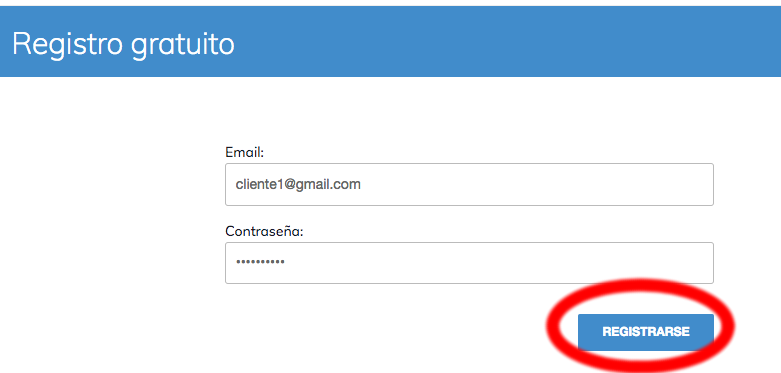
\includegraphics[width=1\linewidth]{register/2.png}
            }
        \end{minipage}

        \item Clic en el link de activación recibido por correo electrónico:

            \medskip
            \begin{minipage}[t]{\linewidth}
            \raggedright
            \adjustbox{valign=t}{%
                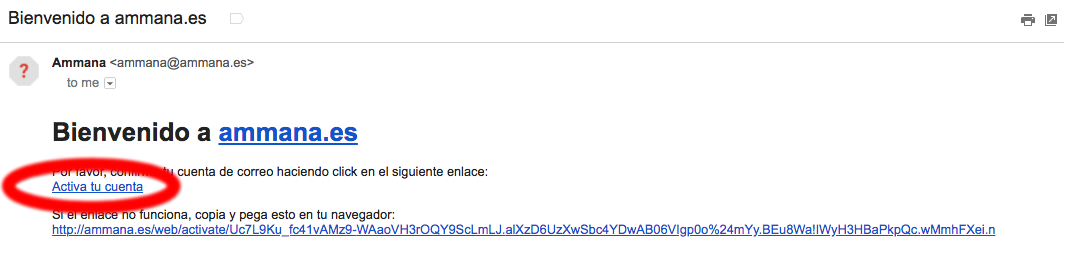
\includegraphics[width=1\linewidth]{register/3.png}
            }
        \end{minipage}

    \end{steps}

%----------------------------------------------------------------------------------------

    \subsubsection{Identificarse}

    \label{sec:login}

    \begin{steps}

        \item Clic en ``Identificarse'' en el menú superior:

            \medskip
            \begin{minipage}[t]{\linewidth}
            \raggedright
            \adjustbox{valign=t}{%
                
\includegraphics[width=1\linewidth]{login/1.png}
            }
        \end{minipage}

        \item Introducir email y contraseña en el formulario de login:

            \medskip
            \begin{minipage}[t]{\linewidth}
            \raggedright
            \adjustbox{valign=t}{%
                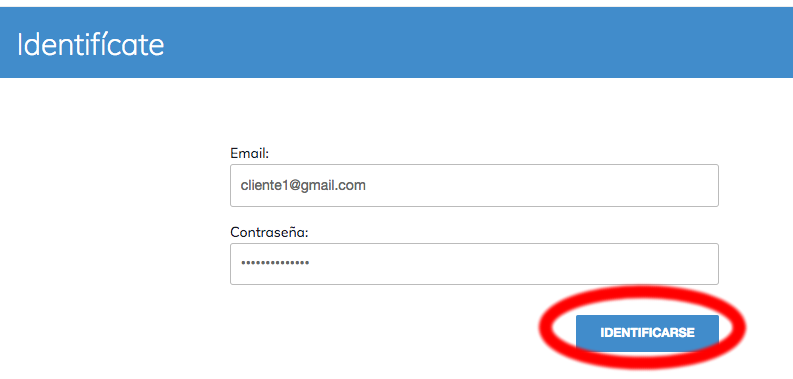
\includegraphics[width=1\linewidth]{login/2.png}
            }
        \end{minipage}

        \item Clic en botón ``Identificarse'':

            \medskip
            \begin{minipage}[t]{\linewidth}
            \raggedright
            \adjustbox{valign=t}{%
                
\includegraphics[width=1\linewidth]{login/3.png}
            }
        \end{minipage}

    \end{steps}

        Si has olvidado tu contraseña, siempre puedes recuperar el acceso a tu cuenta
    siguiendo los pasos indicados en \hyperref[sec:forgot-password]{Recuperar contraseña}.

%----------------------------------------------------------------------------------------

    \subsubsection{Recuperar contraseña}

    \label{sec:forgot-password}

    \begin{steps}

        \item Clic en ``Identificarse'' en el menú superior:

            \medskip
            \begin{minipage}[t]{\linewidth}
            \raggedright
            \adjustbox{valign=t}{%
                
\includegraphics[width=1\linewidth]{forgot-password/1.png}
            }
        \end{minipage}

        \item Clic en ``Olvidé mi contraseña'':

            \medskip
            \begin{minipage}[t]{\linewidth}
            \raggedright
            \adjustbox{valign=t}{%
                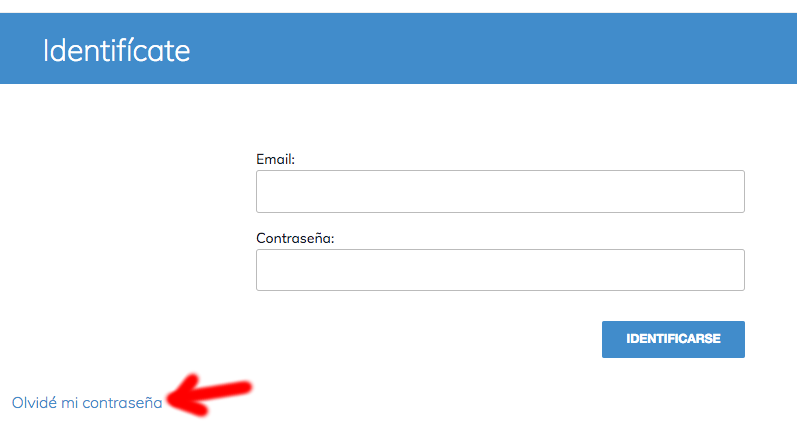
\includegraphics[width=1\linewidth]{forgot-password/2.png}
            }
        \end{minipage}

        \item Introducir email y clic en ``Enviar'':

            \medskip
            \begin{minipage}[t]{\linewidth}
            \raggedright
            \adjustbox{valign=t}{%
                
\includegraphics[width=1\linewidth]{forgot-password/3.png}
            }
        \end{minipage}

        \item Clic en el link de recuperación recibido por correo electrónico:

            \medskip
            \begin{minipage}[t]{\linewidth}
            \raggedright
            \adjustbox{valign=t}{%
                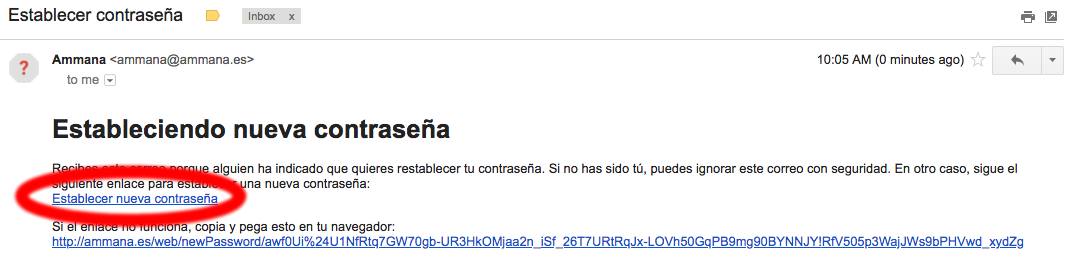
\includegraphics[width=1\linewidth]{forgot-password/4.png}
            }
        \end{minipage}

        \item Introducir nueva contraseña y clic en ``Establecer'':

            \medskip
            \begin{minipage}[t]{\linewidth}
            \raggedright
            \adjustbox{valign=t}{%
                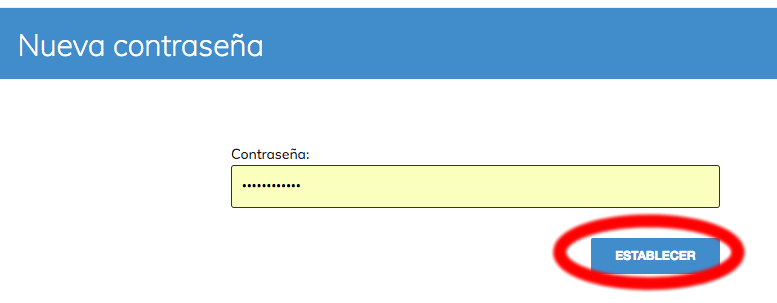
\includegraphics[width=1\linewidth]{forgot-password/5.png}
            }
        \end{minipage}

    \end{steps}

%----------------------------------------------------------------------------------------

    \subsubsection{Modificar datos de perfil de usuario}

    \label{sec:profile}

    \begin{steps}

        \item Clic en ``Mi perfil'' en el menú superior:

            \medskip
            \begin{minipage}[t]{\linewidth}
            \raggedright
            \adjustbox{valign=t}{%
                
\includegraphics[width=1\linewidth]{profile/1.png}
            }
        \end{minipage}

        \item Modificar datos y clic en ``Actualizar'':

            \medskip
            \begin{minipage}[t]{\linewidth}
            \raggedright
            \adjustbox{valign=t}{%
                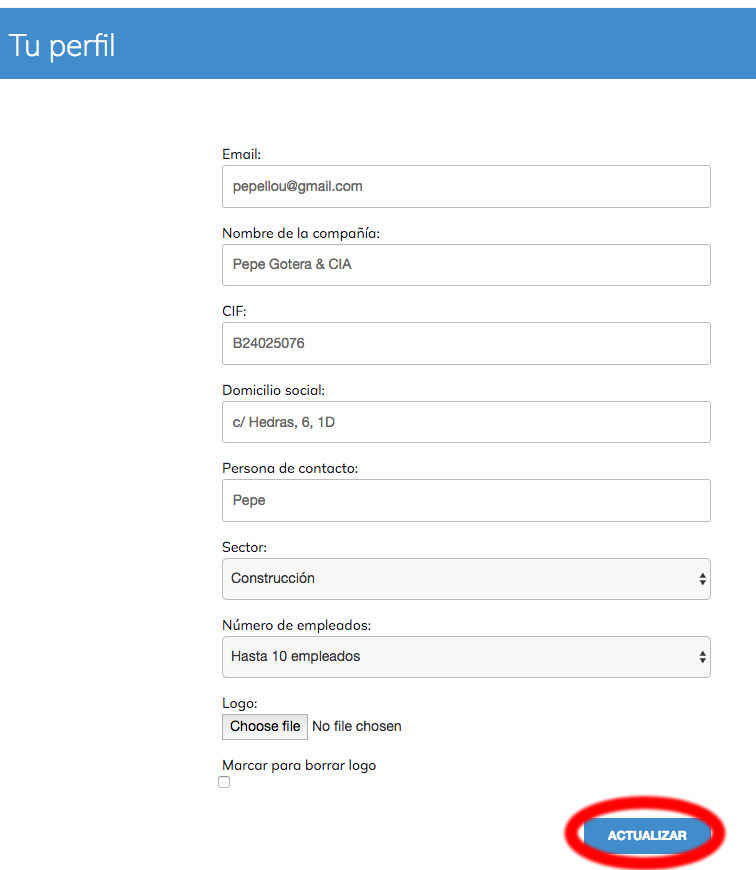
\includegraphics[width=1\linewidth]{profile/2.png}
            }
        \end{minipage}

    \end{steps}
%----------------------------------------------------------------------------------------

    \subsubsection{Cerrar sesión}

    \label{sec:logout}

        Es importante que cierres tu sesión, especialmente si utilizas un ordenador público
    o compartido, para prevenir accesos no autorizados a tu cuenta de ammana.

    \begin{steps}

        \item Clic en ``Cerrar sesión'' en el menú superior:

            \medskip
            \begin{minipage}[t]{\linewidth}
            \raggedright
            \adjustbox{valign=t}{%
                
\includegraphics[width=1\linewidth]{profile/1.png}
            }
        \end{minipage}

        \item Modificar datos y clic en ``Actualizar'':

            \medskip
            \begin{minipage}[t]{\linewidth}
            \raggedright
            \adjustbox{valign=t}{%
                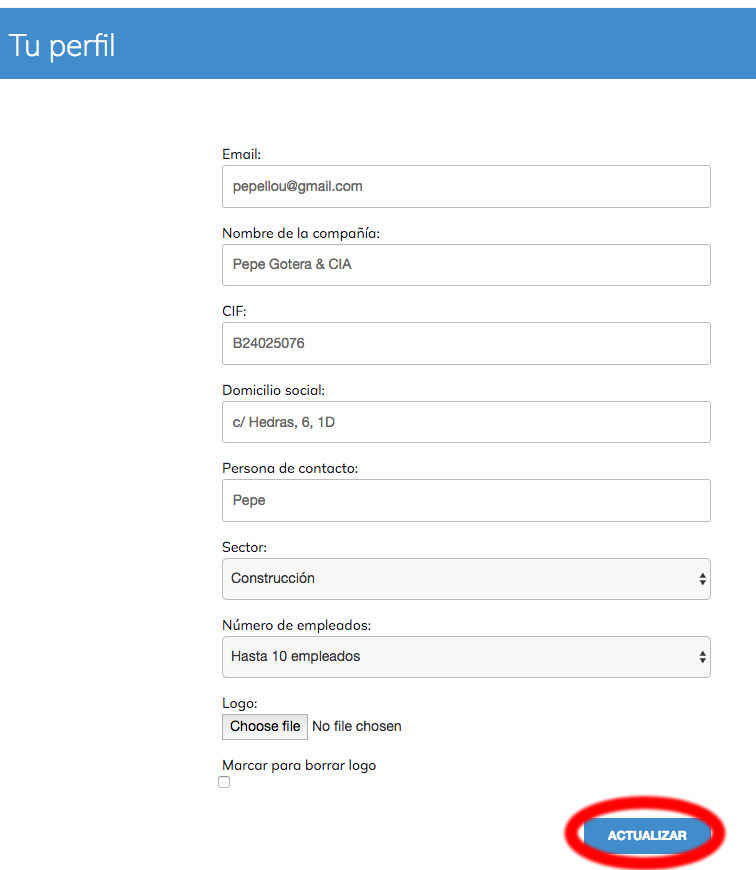
\includegraphics[width=1\linewidth]{profile/2.png}
            }
        \end{minipage}

    \end{steps}

%----------------------------------------------------------------------------------------

    \subsection{Protocolos laborales}

%----------------------------------------------------------------------------------------

    \subsubsection{Comprar protocolo}

    \label{sec:buy-protocol}

    \begin{steps}

        \item Clic en ``Mis protocolos'' en el menú superior:

            \medskip
            \begin{minipage}[t]{\linewidth}
            \raggedright
            \adjustbox{valign=t}{%
                
\includegraphics[width=1\linewidth]{buy-protocol/1.png}
            }
        \end{minipage}

        \item Escoger protocolo en la lista bajo el epígrafe ``Comprar protocolos'':

            \medskip
            \begin{minipage}[t]{\linewidth}
            \raggedright
            \adjustbox{valign=t}{%
                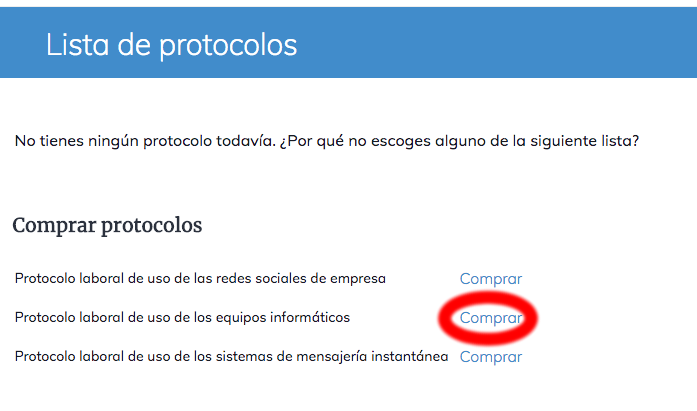
\includegraphics[width=1\linewidth]{buy-protocol/2.png}
            }
        \end{minipage}

        \item Responder todas las preguntas del formulario de preguntas/respuestas sobre el protocolo:

            \medskip
            \begin{minipage}[t]{\linewidth}
            \raggedright
            \adjustbox{valign=t}{%
                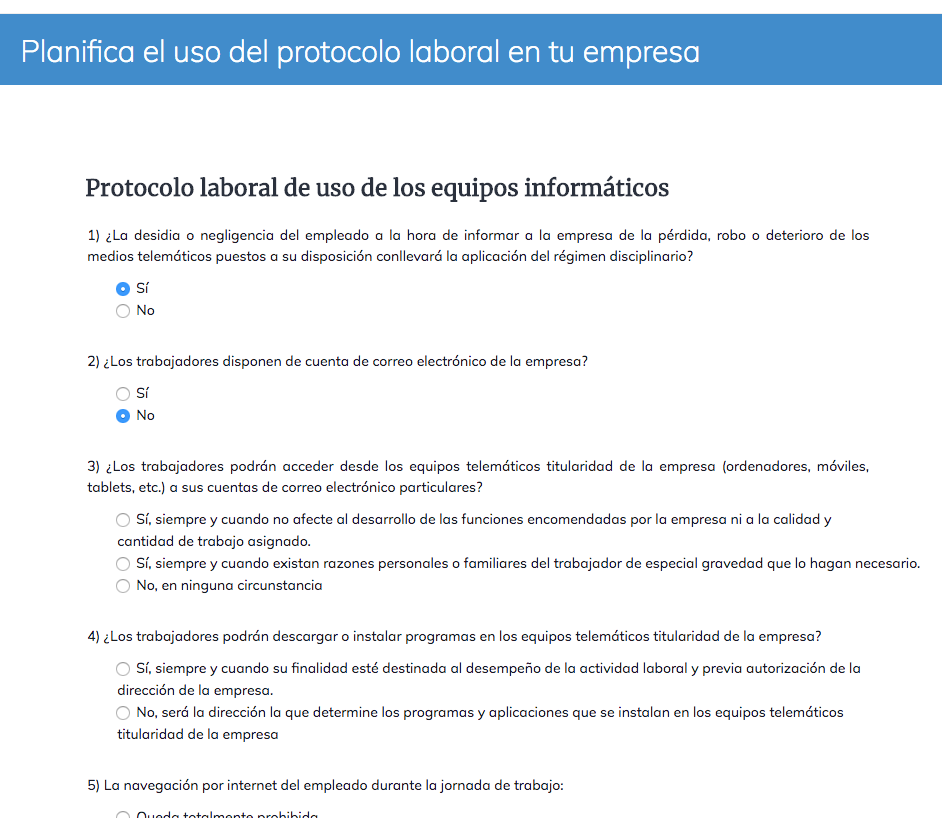
\includegraphics[width=1\linewidth]{buy-protocol/3.png}
            }
        \end{minipage}

        \item Clic en ``Generar protocolo'':

            \medskip
            \begin{minipage}[t]{\linewidth}
            \raggedright
            \adjustbox{valign=t}{%
                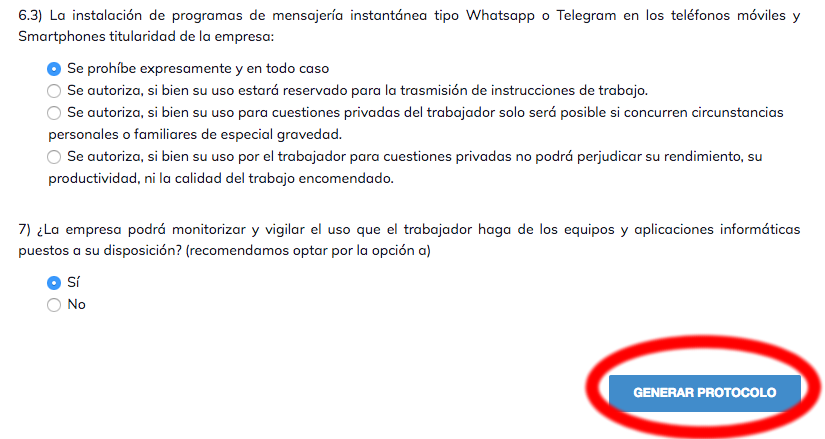
\includegraphics[width=1\linewidth]{buy-protocol/4.png}
            }
        \end{minipage}

        \item Revisar las respuestas (modificarlas en su caso) y clic en ``Confirmar'':

            \medskip
            \begin{minipage}[t]{\linewidth}
            \raggedright
            \adjustbox{valign=t}{%
                
\includegraphics[width=1\linewidth]{buy-protocol/5.png}
            }
        \end{minipage}

        \item El protocolo está pedido. Proceder al \hyperref[sec:paypal]{pago con Paypal}
            o al \hyperref[sec:transfer]{pago por transferencia bancaria}

            \medskip
            \begin{minipage}[t]{\linewidth}
            \raggedright
            \adjustbox{valign=t}{%
                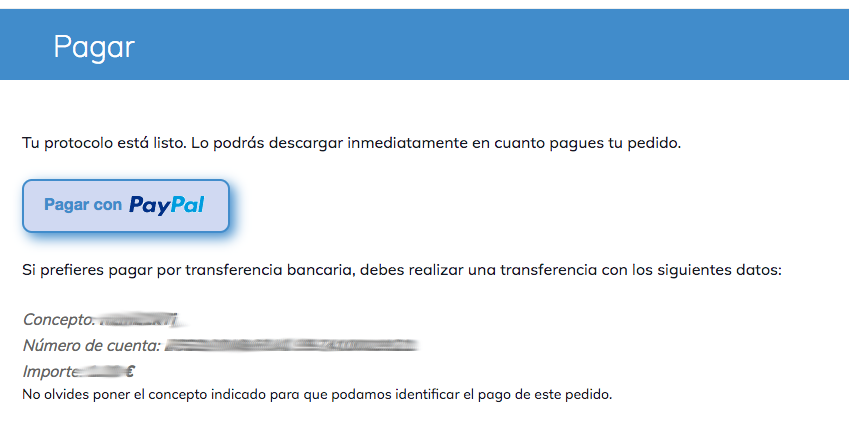
\includegraphics[width=1\linewidth]{buy-protocol/6.png}
            }
        \end{minipage}

    \end{steps}

%----------------------------------------------------------------------------------------

    \subsubsection{Pagar con Paypal}

    \label{sec:paypal}

        Si acabas de pedir un protocolo y estás en la página de pago resultante, pasa directamente
    al paso 3.

    \begin{steps}

        \item Clic en ``Mis protocolos'' en el menú superior:

            \medskip
            \begin{minipage}[t]{\linewidth}
            \raggedright
            \adjustbox{valign=t}{%
                
\includegraphics[width=1\linewidth]{paypal/1.png}
            }
        \end{minipage}

        \item Escoger un protocolo sin pagar y clic en enlace ``pagar'':

            \medskip
            \begin{minipage}[t]{\linewidth}
            \raggedright
            \adjustbox{valign=t}{%
                
\includegraphics[width=1\linewidth]{paypal/2.png}
            }
        \end{minipage}

        \item Clic en botón ``Pagar con PayPal'':

            \medskip
            \begin{minipage}[t]{\linewidth}
            \raggedright
            \adjustbox{valign=t}{%
                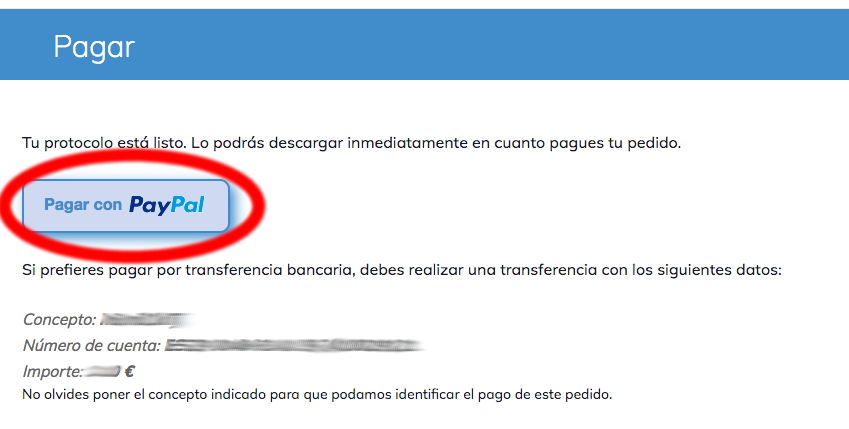
\includegraphics[width=1\linewidth]{paypal/3.png}
            }
        \end{minipage}

        \item Hacer login en Paypal con la cuenta con la que vas a pagar:

            \medskip
            \begin{minipage}[t]{\linewidth}
            \raggedright
            \adjustbox{valign=t}{%
                
\includegraphics[width=1\linewidth]{paypal/4.png}
            }
        \end{minipage}

        \item Clic en botón ``Pagar ahora'':

            \medskip
            \begin{minipage}[t]{\linewidth}
            \raggedright
            \adjustbox{valign=t}{%
                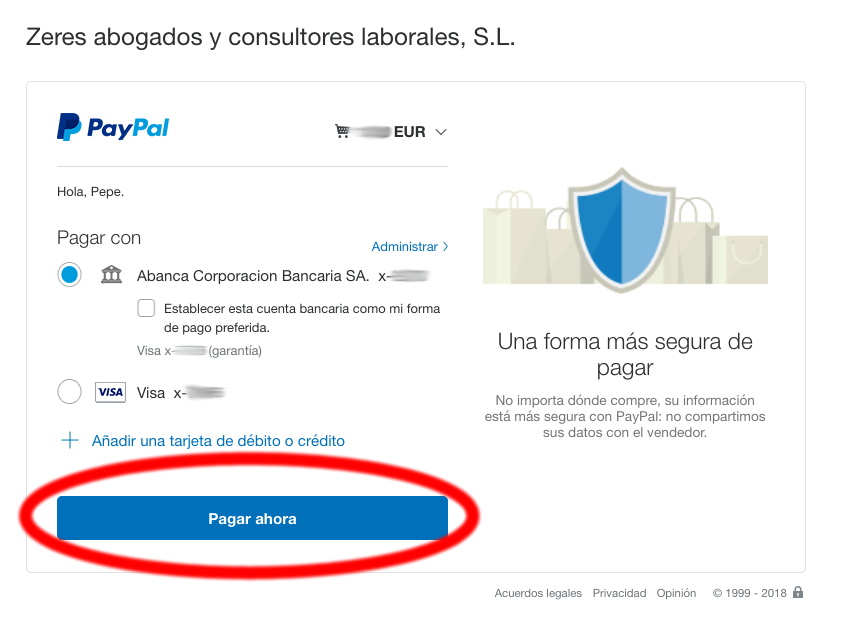
\includegraphics[width=1\linewidth]{paypal/5.png}
            }
        \end{minipage}

    \item Clic en ``Volver al vendedor'' para volver a \textbf{ammana.es}:

            \medskip
            \begin{minipage}[t]{\linewidth}
            \raggedright
            \adjustbox{valign=t}{%
                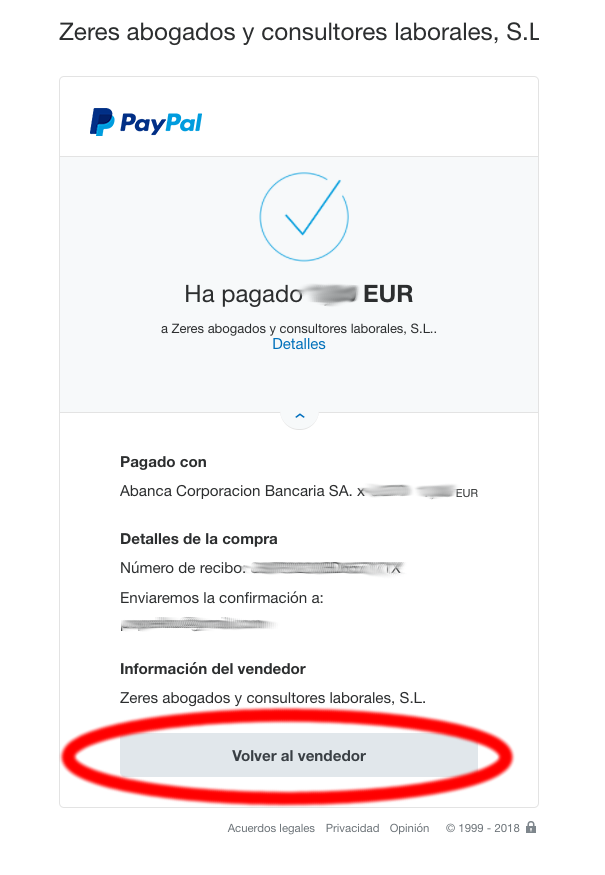
\includegraphics[width=1\linewidth]{paypal/6.png}
            }
        \end{minipage}

    \end{steps}

%----------------------------------------------------------------------------------------

    \subsubsection{Pagar por transferencia bancaria}

    \label{sec:transfer}

        Si acabas de pedir un protocolo y estás en la página de pago resultante, pasa directamente
    al paso 3.

    \begin{steps}

        \item Clic en ``Mis protocolos'' en el menú superior:

            \medskip
            \begin{minipage}[t]{\linewidth}
            \raggedright
            \adjustbox{valign=t}{%
                
\includegraphics[width=1\linewidth]{transfer/1.png}
            }
        \end{minipage}

        \item Escoger un protocolo sin pagar y clic en enlace ``pagar'':

            \medskip
            \begin{minipage}[t]{\linewidth}
            \raggedright
            \adjustbox{valign=t}{%
                
\includegraphics[width=1\linewidth]{transfer/2.png}
            }
        \end{minipage}

        \item Usa los datos indicados para realizar tu transferencia:

            \medskip
            \begin{minipage}[t]{\linewidth}
            \raggedright
            \adjustbox{valign=t}{%
                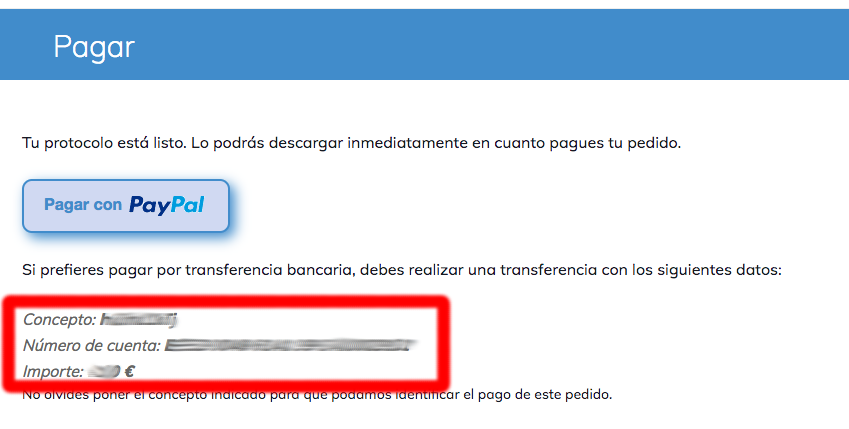
\includegraphics[width=1\linewidth]{transfer/3.png}
            }
        \end{minipage}

    \end{steps}

            Las transferencias bancarias pueden tardar hasta 2 días en hacerse efectivas, y tras ello
        el personal de \textbf{ammana.es} tiene que procesar manualmente las transferencias recibidas,
        por lo que pueden pasar algunos días hasta que tengas tu protocolo disponible.

%----------------------------------------------------------------------------------------

    \subsubsection{Descargar protocolo, instrucciones y recibí}

    \label{sec:download-protocol}

        Siempre vas a tener disponibles todos tus documentos en la sección ``Mis protocolos''.

    \begin{steps}

        \item Clic en ``Mis protocolos'' en el menú superior:

            \medskip
            \begin{minipage}[t]{\linewidth}
            \raggedright
            \adjustbox{valign=t}{%
                
\includegraphics[width=1\linewidth]{download-protocol/1.png}
            }
        \end{minipage}

        \item Escoger un protocolo y clic en enlace ``Protocolo'' para descargarlo:

            \medskip
            \begin{minipage}[t]{\linewidth}
            \raggedright
            \adjustbox{valign=t}{%
                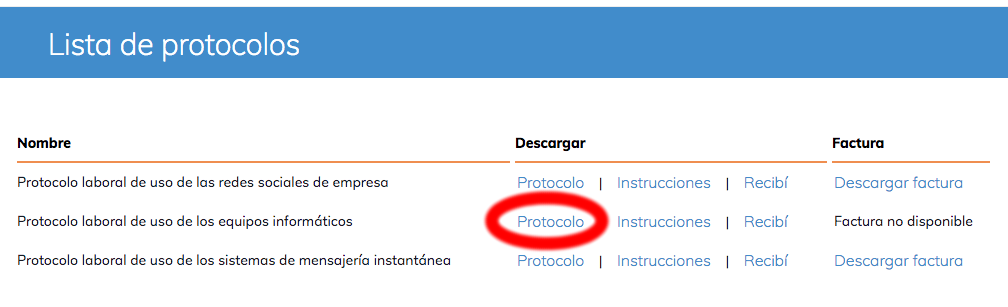
\includegraphics[width=1\linewidth]{download-protocol/2.png}
            }
        \end{minipage}

        \item Clic en enlace ``Instrucciones'' para descargar documento con instrucciones de uso del protocolo:

            \medskip
            \begin{minipage}[t]{\linewidth}
            \raggedright
            \adjustbox{valign=t}{%
                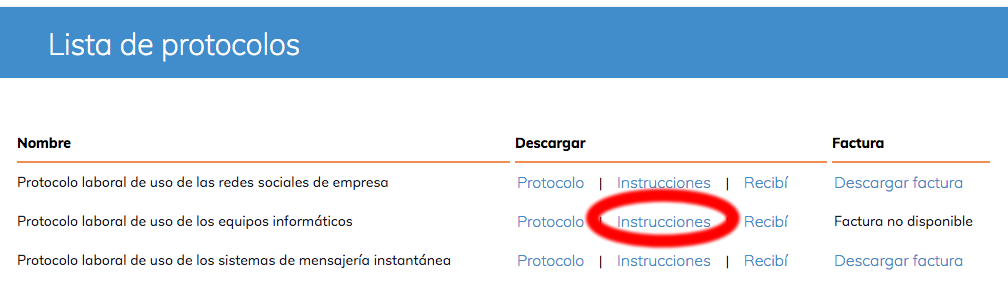
\includegraphics[width=1\linewidth]{download-protocol/3.png}
            }
        \end{minipage}

        \item Clic en enlace ``Recibí'' para descargar modelo de recibí del protocolo laboral:

            \medskip
            \begin{minipage}[t]{\linewidth}
            \raggedright
            \adjustbox{valign=t}{%
                
\includegraphics[width=1\linewidth]{download-protocol/4.png}
            }
        \end{minipage}

    \end{steps}

%----------------------------------------------------------------------------------------

    \subsubsection{Descargar facturas}

    \label{sec:download-invoices}

            Tanto si pagas por Paypal como por transferencia, siempre vas a tener disponibles
        las facturas de tus pedidos en la sección ``Mis facturas'':

    \begin{steps}

        \item Clic en ``Mis facturas'' en el menú superior:

            \medskip
            \begin{minipage}[t]{\linewidth}
            \raggedright
            \adjustbox{valign=t}{%
                
\includegraphics[width=1\linewidth]{download-invoices/1.png}
            }
        \end{minipage}

        \item Escoger una factura y clic en enlace ``Descargar factura'' para descargarla:

            \medskip
            \begin{minipage}[t]{\linewidth}
            \raggedright
            \adjustbox{valign=t}{%
                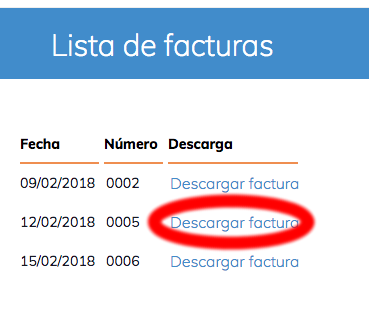
\includegraphics[width=1\linewidth]{download-invoices/2.png}
            }
        \end{minipage}

    \end{steps}

            Alternativamente puedes acceder a cada factura desde la lista de protocolos:

    \begin{steps}

        \item Clic en ``Mis protocolos'' en el menú superior:

            \medskip
            \begin{minipage}[t]{\linewidth}
            \raggedright
            \adjustbox{valign=t}{%
                
\includegraphics[width=1\linewidth]{download-invoices/3.png}
            }
        \end{minipage}

        \item Escoger un protocolo y clic en enlace ``Descargar factura'' para descargarla:

            \medskip
            \begin{minipage}[t]{\linewidth}
            \raggedright
            \adjustbox{valign=t}{%
                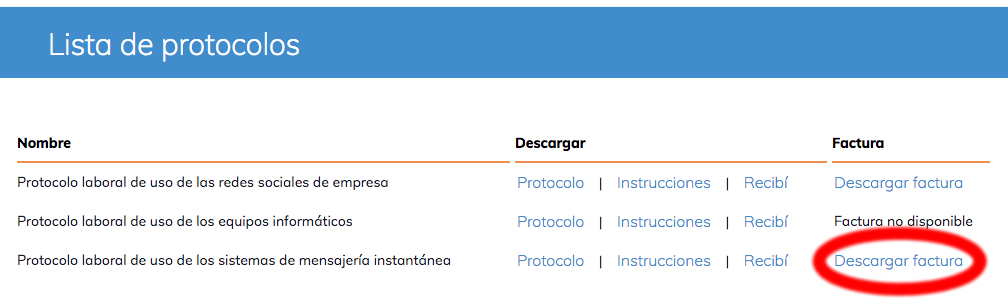
\includegraphics[width=1\linewidth]{download-invoices/4.png}
            }
        \end{minipage}

    \end{steps}

%----------------------------------------------------------------------------------------

\end{document}
